\documentclass[11pt, a4paper]{article}\usepackage[]{graphicx}\usepackage[]{xcolor}
% maxwidth is the original width if it is less than linewidth
% otherwise use linewidth (to make sure the graphics do not exceed the margin)
\makeatletter
\def\maxwidth{ %
  \ifdim\Gin@nat@width>\linewidth
    \linewidth
  \else
    \Gin@nat@width
  \fi
}
\makeatother

\definecolor{fgcolor}{rgb}{0.345, 0.345, 0.345}
\newcommand{\hlnum}[1]{\textcolor[rgb]{0.686,0.059,0.569}{#1}}%
\newcommand{\hlsng}[1]{\textcolor[rgb]{0.192,0.494,0.8}{#1}}%
\newcommand{\hlcom}[1]{\textcolor[rgb]{0.678,0.584,0.686}{\textit{#1}}}%
\newcommand{\hlopt}[1]{\textcolor[rgb]{0,0,0}{#1}}%
\newcommand{\hldef}[1]{\textcolor[rgb]{0.345,0.345,0.345}{#1}}%
\newcommand{\hlkwa}[1]{\textcolor[rgb]{0.161,0.373,0.58}{\textbf{#1}}}%
\newcommand{\hlkwb}[1]{\textcolor[rgb]{0.69,0.353,0.396}{#1}}%
\newcommand{\hlkwc}[1]{\textcolor[rgb]{0.333,0.667,0.333}{#1}}%
\newcommand{\hlkwd}[1]{\textcolor[rgb]{0.737,0.353,0.396}{\textbf{#1}}}%
\let\hlipl\hlkwb

\usepackage{framed}
\makeatletter
\newenvironment{kframe}{%
 \def\at@end@of@kframe{}%
 \ifinner\ifhmode%
  \def\at@end@of@kframe{\end{minipage}}%
  \begin{minipage}{\columnwidth}%
 \fi\fi%
 \def\FrameCommand##1{\hskip\@totalleftmargin \hskip-\fboxsep
 \colorbox{shadecolor}{##1}\hskip-\fboxsep
     % There is no \\@totalrightmargin, so:
     \hskip-\linewidth \hskip-\@totalleftmargin \hskip\columnwidth}%
 \MakeFramed {\advance\hsize-\width
   \@totalleftmargin\z@ \linewidth\hsize
   \@setminipage}}%
 {\par\unskip\endMakeFramed%
 \at@end@of@kframe}
\makeatother

\definecolor{shadecolor}{rgb}{.97, .97, .97}
\definecolor{messagecolor}{rgb}{0, 0, 0}
\definecolor{warningcolor}{rgb}{1, 0, 1}
\definecolor{errorcolor}{rgb}{1, 0, 0}
\newenvironment{knitrout}{}{} % an empty environment to be redefined in TeX

\usepackage{alltt}

\usepackage[top=1 in, bottom = 1 in, left = 1 in, right = 1 in ]{geometry}

\usepackage{amsmath, amssymb, amsfonts}
\usepackage{enumerate}

\title{Histogram}
\author{Ananda Biswas}
\date{}
\IfFileExists{upquote.sty}{\usepackage{upquote}}{}
\begin{document}

\maketitle

\begin{knitrout}
\definecolor{shadecolor}{rgb}{0.969, 0.969, 0.969}\color{fgcolor}\begin{kframe}
\begin{alltt}
\hlkwd{hist}\hldef{(mtcars}\hlopt{$}\hldef{mpg,}
     \hlkwc{xlab} \hldef{=} \hlsng{"Classes"}\hldef{,}
     \hlkwc{ylab} \hldef{=} \hlsng{"Frequencies"}\hldef{,}
     \hlkwc{col} \hldef{=} \hlsng{"orange"}\hldef{)}
\end{alltt}
\end{kframe}
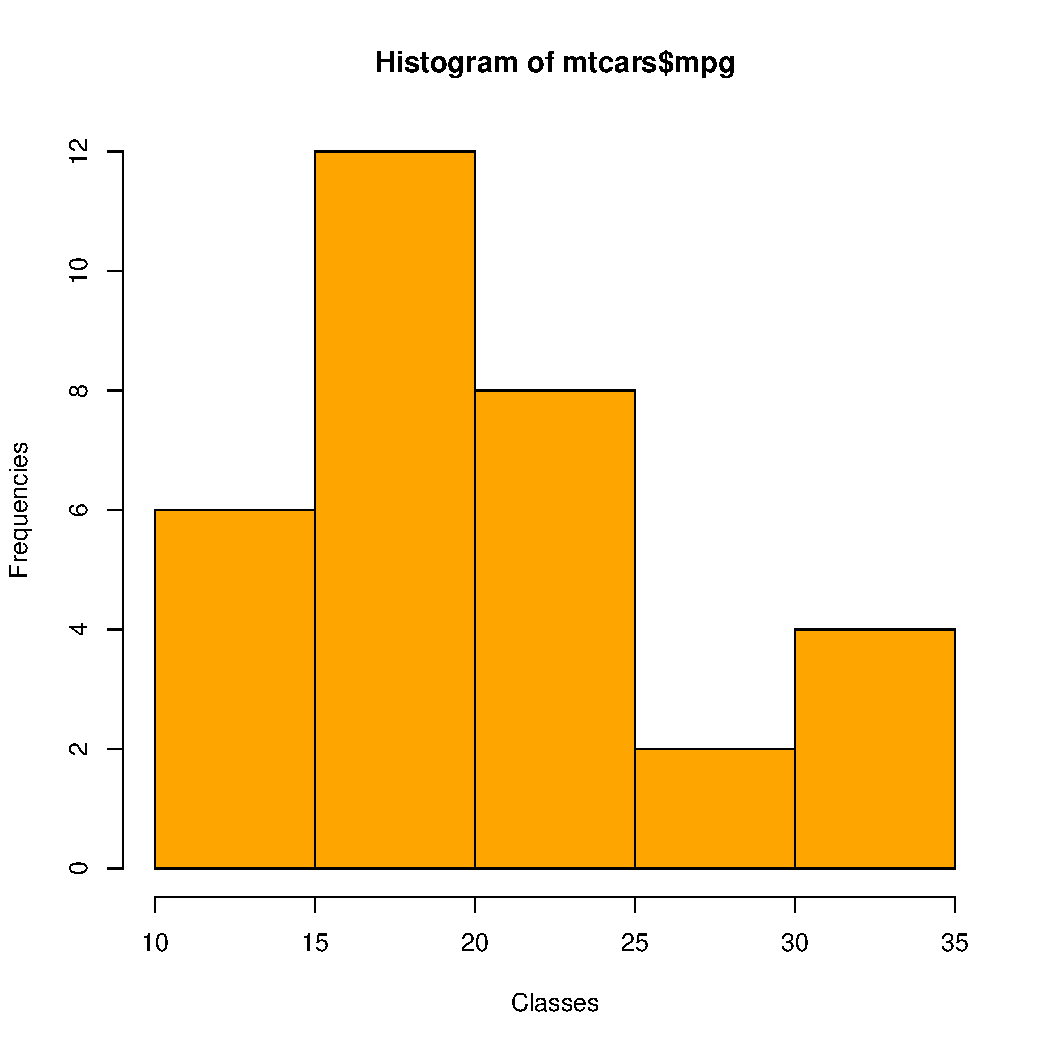
\includegraphics[width=\maxwidth]{figure/unnamed-chunk-1-1} 
\end{knitrout}

\newpage

$\bullet$ When \textbf{breaks} is a number, it denotes the number of classes, i.e. the number of vertical cells in the diagram.
\begin{knitrout}
\definecolor{shadecolor}{rgb}{0.969, 0.969, 0.969}\color{fgcolor}\begin{kframe}
\begin{alltt}
\hlkwd{hist}\hldef{(mtcars}\hlopt{$}\hldef{mpg,}
     \hlkwc{xlab} \hldef{=} \hlsng{"Classes"}\hldef{,}
     \hlkwc{ylab} \hldef{=} \hlsng{"Frequencies"}\hldef{,}
     \hlkwc{col} \hldef{=} \hlsng{"orange"}\hldef{,}
     \hlkwc{breaks} \hldef{=} \hlnum{10}\hldef{)}
\end{alltt}
\end{kframe}
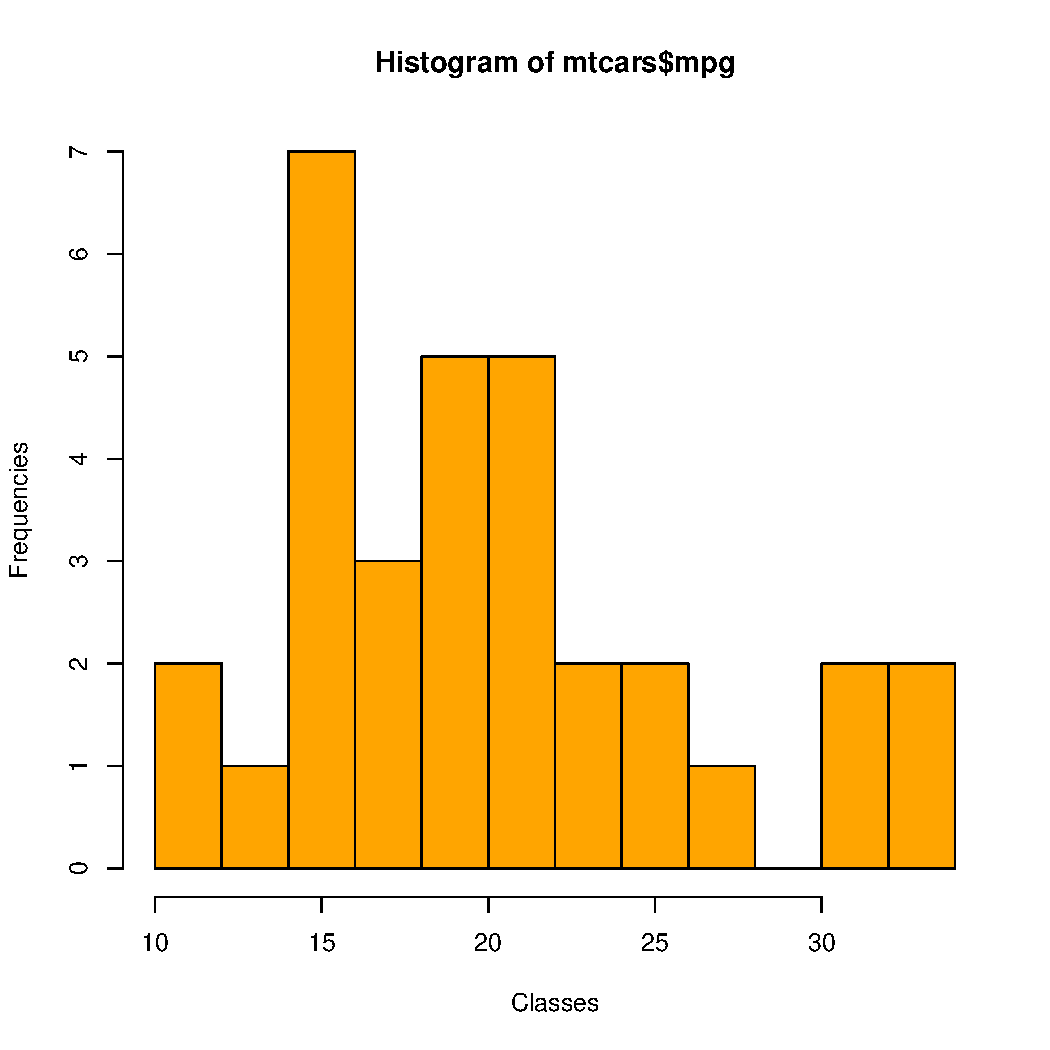
\includegraphics[width=\maxwidth]{figure/unnamed-chunk-2-1} 
\end{knitrout}

\newpage

$\bullet$ When \textbf{breaks} is a vector, it gives the breakpoints between the histogram cells.
\begin{knitrout}
\definecolor{shadecolor}{rgb}{0.969, 0.969, 0.969}\color{fgcolor}\begin{kframe}
\begin{alltt}
\hlkwd{range}\hldef{(mtcars}\hlopt{$}\hldef{mpg)}
\end{alltt}
\begin{verbatim}
## [1] 10.4 33.9
\end{verbatim}
\begin{alltt}
\hldef{breaks_vector} \hlkwb{<-} \hlkwd{seq}\hldef{(}\hlkwc{from} \hldef{=} \hlnum{10}\hldef{,} \hlkwc{to} \hldef{=} \hlnum{34}\hldef{,} \hlkwc{by} \hldef{=} \hlnum{3}\hldef{)}

\hlkwd{hist}\hldef{(mtcars}\hlopt{$}\hldef{mpg,}
     \hlkwc{xlab} \hldef{=} \hlsng{"Classes"}\hldef{,}
     \hlkwc{ylab} \hldef{=} \hlsng{"Frequencies"}\hldef{,}
     \hlkwc{col} \hldef{=} \hlsng{"orange"}\hldef{,}
     \hlkwc{breaks} \hldef{= breaks_vector)}
\end{alltt}
\end{kframe}
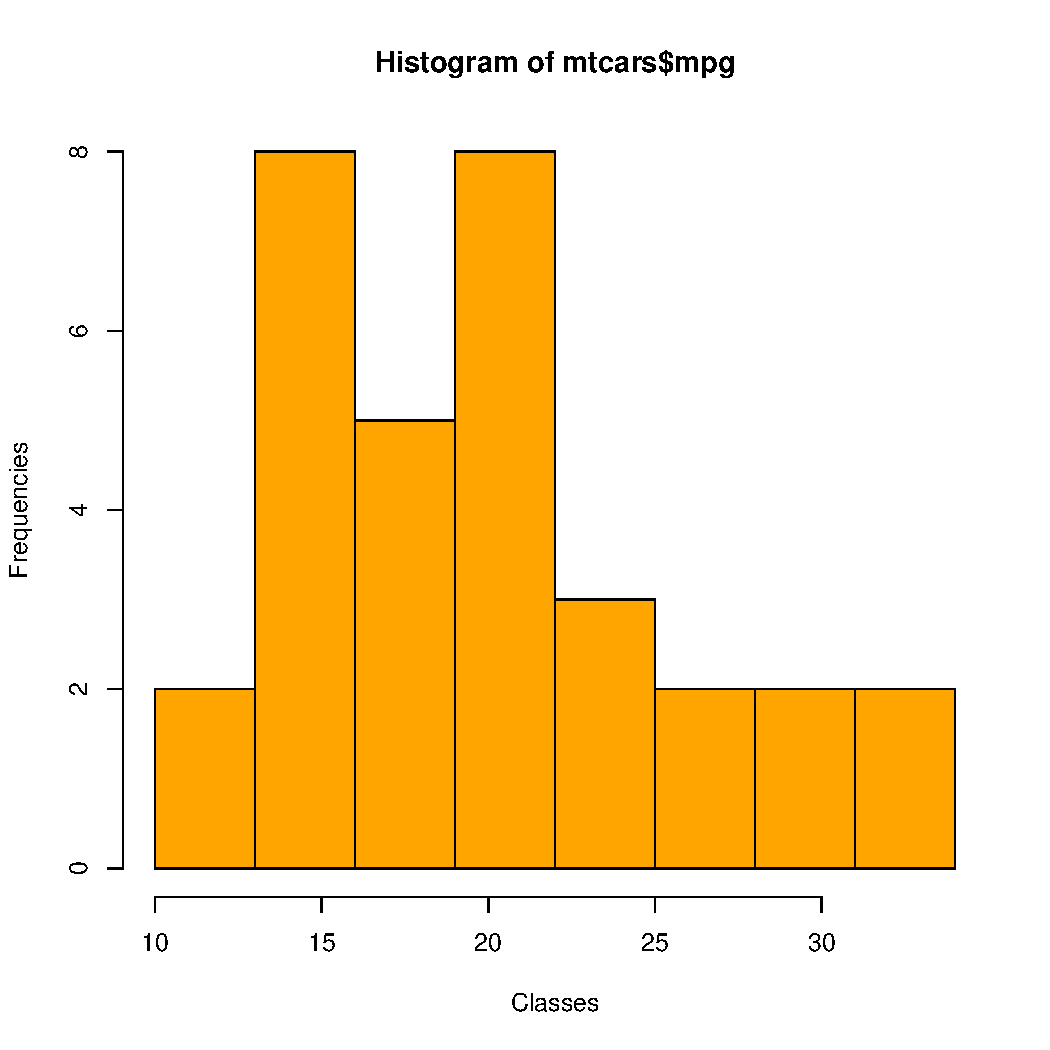
\includegraphics[width=\maxwidth]{figure/unnamed-chunk-3-1} 
\end{knitrout}

\newpage

$\bullet$ \textit{xaxp = c(10, 34, 8)} displays 8 equidistant breakpoints in the histogram, starting from 10 up to 34. \\

\hspace{0.5cm} \textit{xaxt} argument and \textit{axis()} function can also be used here.

\begin{knitrout}
\definecolor{shadecolor}{rgb}{0.969, 0.969, 0.969}\color{fgcolor}\begin{kframe}
\begin{alltt}
\hldef{breaks_vector} \hlkwb{<-} \hlkwd{seq}\hldef{(}\hlkwc{from} \hldef{=} \hlnum{10}\hldef{,} \hlkwc{to} \hldef{=} \hlnum{34}\hldef{,} \hlkwc{by} \hldef{=} \hlnum{3}\hldef{)}

\hlkwd{hist}\hldef{(mtcars}\hlopt{$}\hldef{mpg,}
     \hlkwc{xlab} \hldef{=} \hlsng{"Classes"}\hldef{,}
     \hlkwc{ylab} \hldef{=} \hlsng{"Frequencies"}\hldef{,}
     \hlkwc{col} \hldef{=} \hlsng{"orange"}\hldef{,}
     \hlkwc{breaks} \hldef{= breaks_vector,}
     \hlkwc{xaxp} \hldef{=} \hlkwd{c}\hldef{(}\hlnum{10}\hldef{,} \hlnum{34}\hldef{,} \hlnum{8}\hldef{))}
\end{alltt}
\end{kframe}
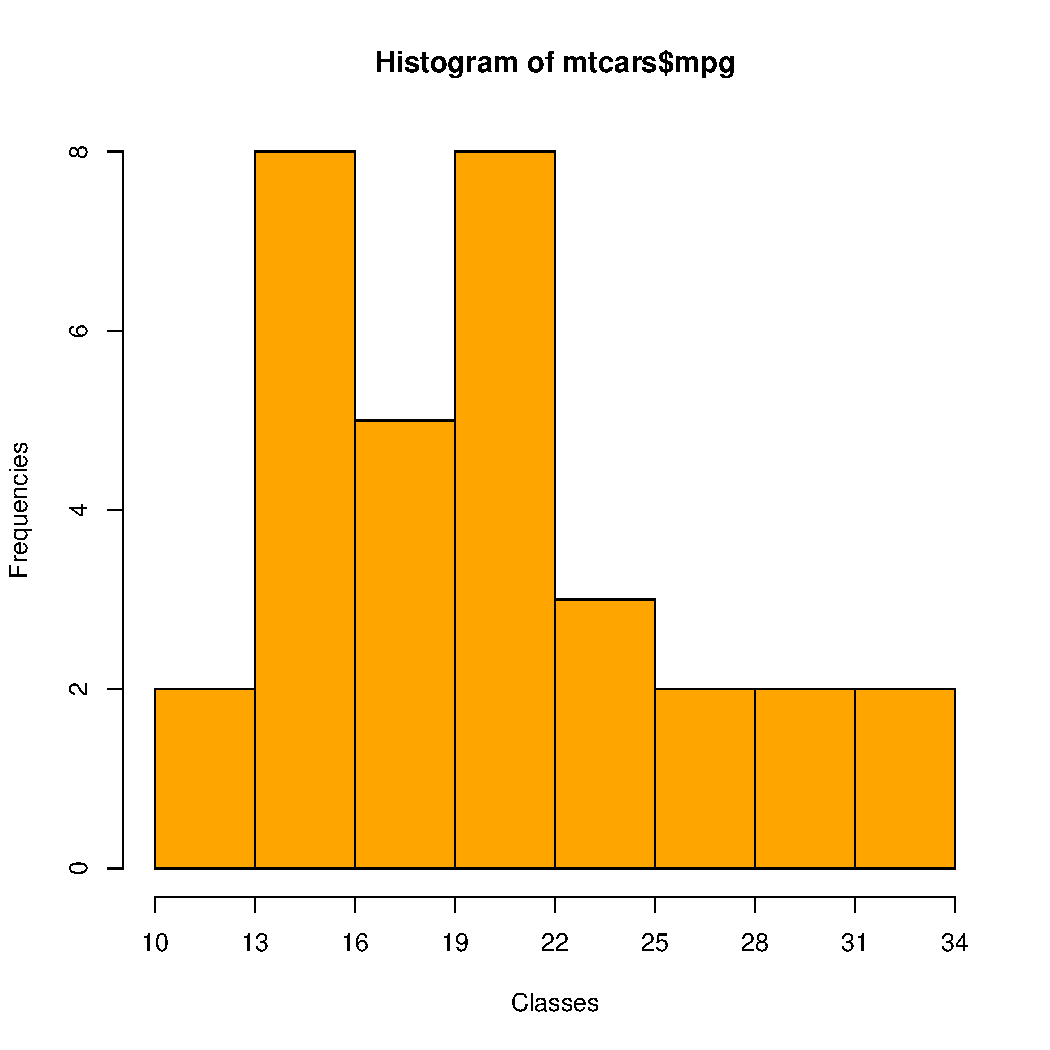
\includegraphics[width=\maxwidth]{figure/unnamed-chunk-4-1} 
\end{knitrout}

\newpage

$\bullet$ Histogram with frequency density
\begin{knitrout}
\definecolor{shadecolor}{rgb}{0.969, 0.969, 0.969}\color{fgcolor}\begin{kframe}
\begin{alltt}
\hlkwd{hist}\hldef{(mtcars}\hlopt{$}\hldef{mpg,}
     \hlkwc{xlab} \hldef{=} \hlsng{"Classes"}\hldef{,}
     \hlkwc{ylab} \hldef{=} \hlsng{"Frequency Densities"}\hldef{,}
     \hlkwc{col} \hldef{=} \hlsng{"orange"}\hldef{,}
     \hlkwc{probability} \hldef{=} \hlnum{TRUE}\hldef{)}
\end{alltt}
\end{kframe}
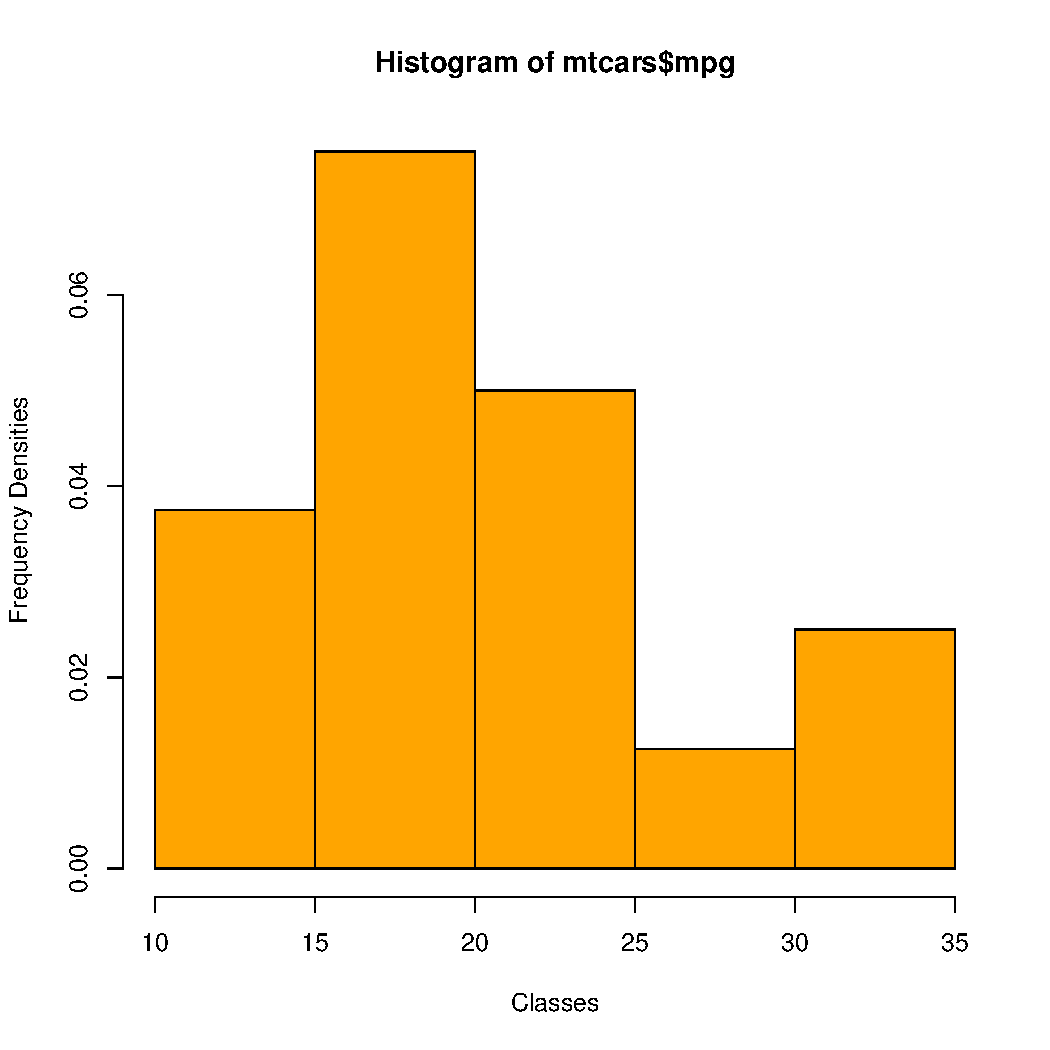
\includegraphics[width=\maxwidth]{figure/unnamed-chunk-5-1} 
\end{knitrout}

\newpage

\begin{knitrout}
\definecolor{shadecolor}{rgb}{0.969, 0.969, 0.969}\color{fgcolor}\begin{kframe}
\begin{alltt}
\hlkwd{hist}\hldef{(quakes}\hlopt{$}\hldef{mag,} \hlkwc{probability} \hldef{=} \hlnum{TRUE}\hldef{)}
\hlkwd{lines}\hldef{(}\hlkwd{density}\hldef{(quakes}\hlopt{$}\hldef{mag))}
\end{alltt}
\end{kframe}
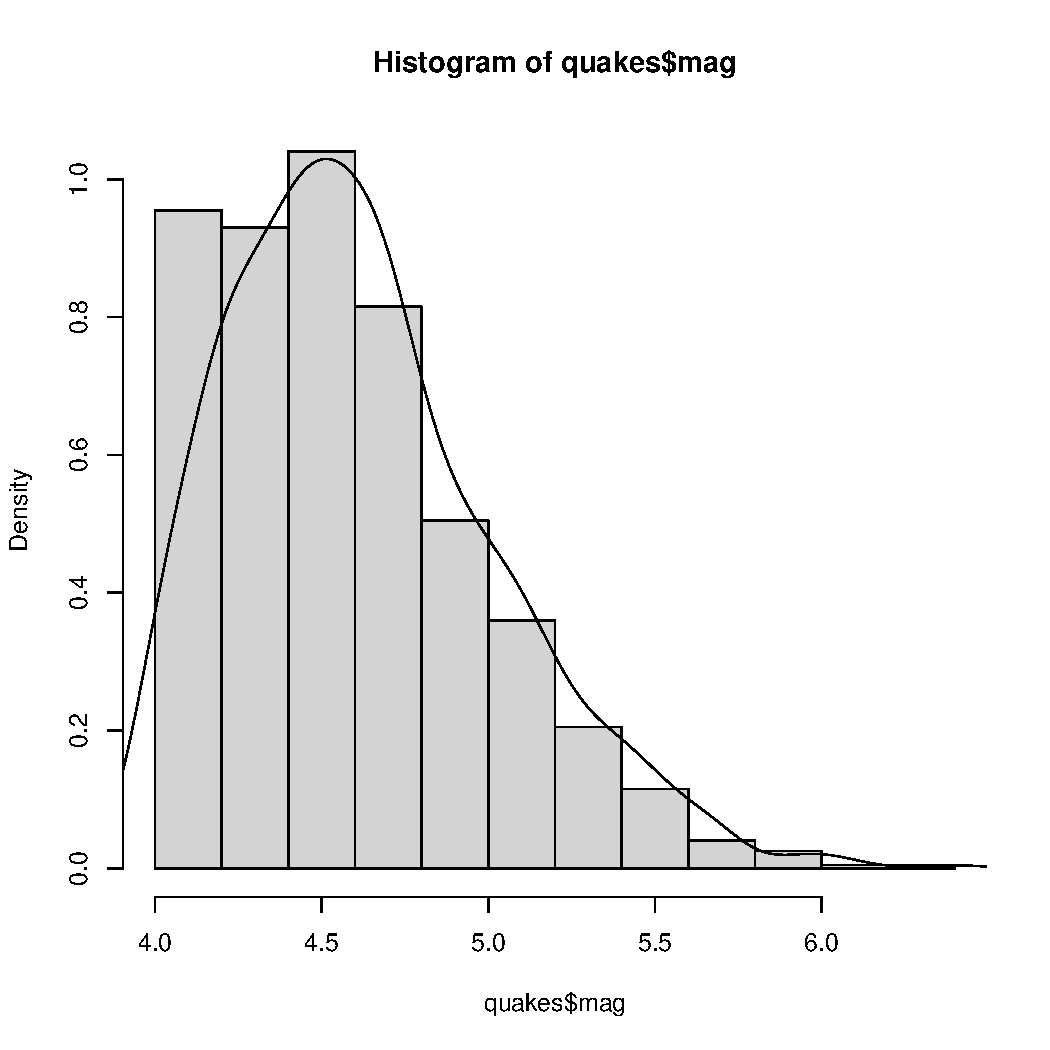
\includegraphics[width=\maxwidth]{figure/unnamed-chunk-6-1} 
\end{knitrout}

\newpage

$\bullet$ A plot that resembles a ``discrete histogram" :
\begin{knitrout}
\definecolor{shadecolor}{rgb}{0.969, 0.969, 0.969}\color{fgcolor}\begin{kframe}
\begin{alltt}
\hlkwd{plot}\hldef{(}\hlkwd{table}\hldef{(airquality}\hlopt{$}\hldef{Temp),}
     \hlkwc{type} \hldef{=} \hlsng{"h"}\hldef{,}
     \hlkwc{lwd} \hldef{=} \hlnum{5}\hldef{,}
     \hlkwc{xlab} \hldef{=} \hlsng{"Temperatures"}\hldef{,}
     \hlkwc{ylab} \hldef{=} \hlsng{"Frequencies"}\hldef{,}
     \hlkwc{main} \hldef{=} \hlsng{"Frequencies of the Temperatures"}\hldef{,}
     \hlkwc{col} \hldef{=} \hlsng{"blue"}\hldef{)}
\end{alltt}
\end{kframe}
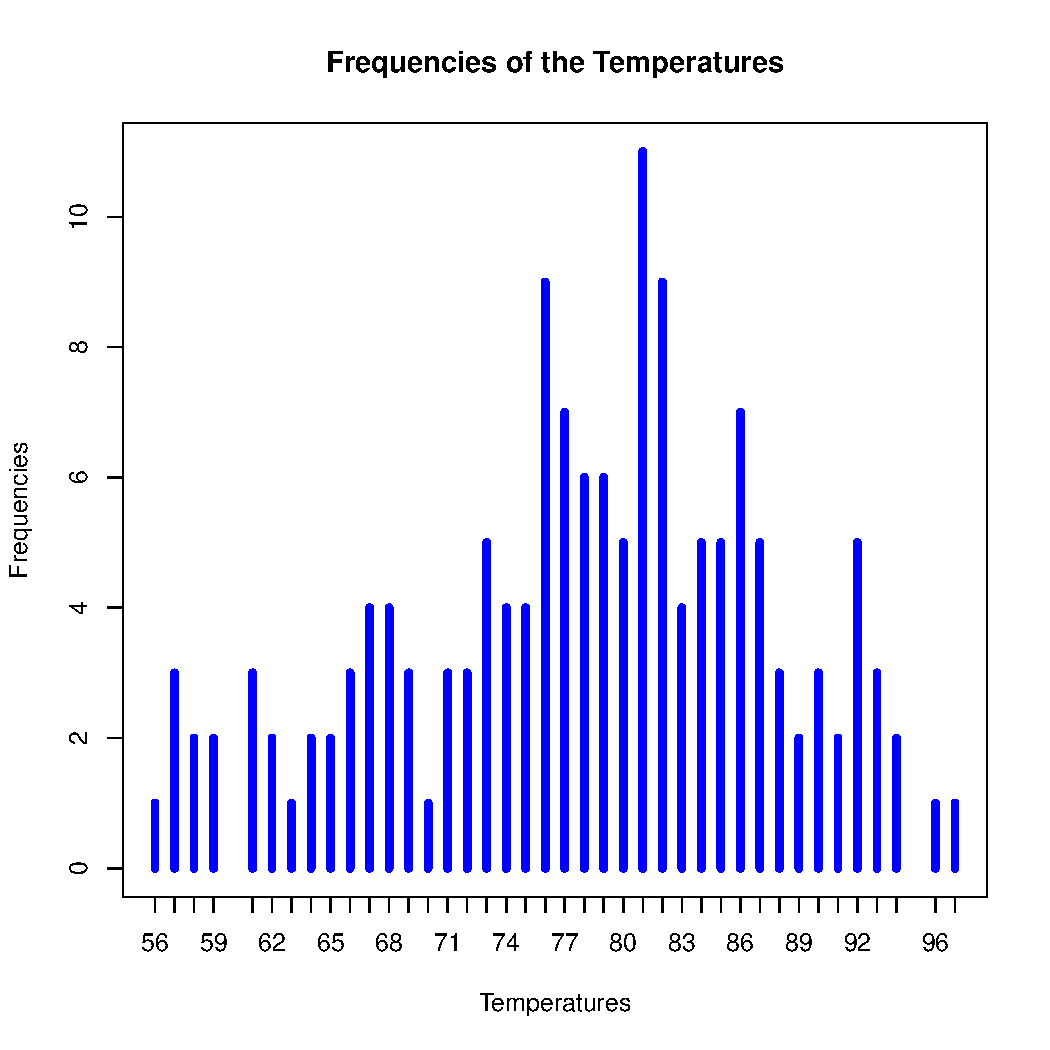
\includegraphics[width=\maxwidth]{figure/unnamed-chunk-7-1} 
\end{knitrout}

\end{document}
